\section{Basic Introduction}

In this chapter, a brief overview of the classical SIR model developed by Kermack-Mckendrick [1] in 1927, will be given. This model attempts to estimate and predict the distribution and number of infections for an infectious disease. The SIR model serves as the most primary ground in developing more elaborate and complicated epidemiological models. \\

The SIR model categorizes the whole population into three compartments. First, the susceptible compartment S, secondly the infected and infectious compartment I, and finally the recovered compartment R. \\

\begin{itemize}
	\item The susceptible population S denotes the number of healthy people who are not yet infected but are prone or vulnerable to infection.  \\
	
	\item The infectious population I denotes the people who are already infected and sick from the susceptible population. These people are also infectious and are waiting to be recovered.  \\
	
	\item And lastly, the recovered population R, who are assumed to be recovered from the disease.
\end{itemize}

This model can be visualized in the picture below--- \\

\begin{figure}[H]
\centering

\includegraphics[scale=1.0]{SIR.png}
\caption{SIR Model}
\label{fig:SIR Model}
\end{figure}

Here, the individuals transfer from the susceptible compartment S to the infectious compartment I at a rate of \textbeta SI, where \textbeta \ is a positive constant and the transmission rate from S to I. And finally, individuals transfer from the infectious compartment I to the recovered compartment R at a rate of \textalpha I, where \textalpha \ is again a positive constant and the recovery rate for individuals from I to R. Here, it is important to note that, the transmission rate from the susceptible population S to the infected population I depends both on the susceptible and infectious compartments and hence, the rate is defined as \textbeta SI. \\

So the model can be summarized as a system of ordinary differential equations as given below--- \\

\begin{equation}
\begin{aligned}
&S^{\prime}(t)=-\beta SI \\
&I^{\prime}(t)=\beta SI - \alpha I \\
&R^{\prime}(t)=\alpha I \\
\end{aligned}
\end{equation}

Here, all the variables S, I, and R are functions of time, which means that they only change their values with respect to the time. It is also crucial that, the size of the whole population at any given time t, is the sum of all the individuals from the susceptible, infectious, and recovered compartments. That means--- \\

$ N=S (t)+I (t)+R (t) $
\\

Some other important fundamental characteristics of this model are--- \\

\begin{itemize}
	\item The whole population is closed. That means the number of total individuals remains constant within the given time t, i.e. $N^{\prime}(t) = S^{\prime}(t)+I^{\prime} (t)+R^{\prime} (t)= 0$ and $N=S (0)+I (0)+R (0)$. The population is continuous in time. \\
	
	\item All the individuals receive immunity as soon as they enter the recovered compartment R, either by immunity from reinfection or by death. So the possibility for reinfection is omitted. \\
	
	\item The duration of the disease spread or epidemic is smaller than the lifespan of the population. \\
	
	\item The incubation period [19] for the disease is negligible. So any individual who gets infected is moved immediately to the infectious compartment I. \\
	
	\item The population is homogeneously [20] mixed. All the individuals within the population have an equal probability of getting into contact with each other and getting infected. \\
	
	\item The unit of transmission rate \textbeta \ = 1/(population size $\times$ unit of time), and \\
The unit of recovery rate \textalpha \ = 1/(unit of time) [3]

\end{itemize}

\pagebreak
\section{Example}

A sample real life epidemic case can be solved here with the SIR model using python. For this, let us consider a dataset from an influenza epidemic that occurred in a boys boarding school in the north of England in 1978 [21], [22]. \\

In this case, the epidemic lasted for two weeks. There were in total of 763 boys who were residents in that boarding school, including one who was infected initially. \\

So we can set the initial conditions--- \\
\noindent Initial susceptible, S (0) = 762 \\
Initial infected, I (0) = 1 \\
Initial recovered, R (0) = 0 \\
Time period, t = 14 days \\
Step size = 1 \\

And the transmission rate as well as recovery rate values are taken from [5] \\
\textbeta \ = 0.00218 \\
\textalpha \ = 0.441 \\

Now it is possible to model these data using python. \\

\begin{figure}[H]
\centering
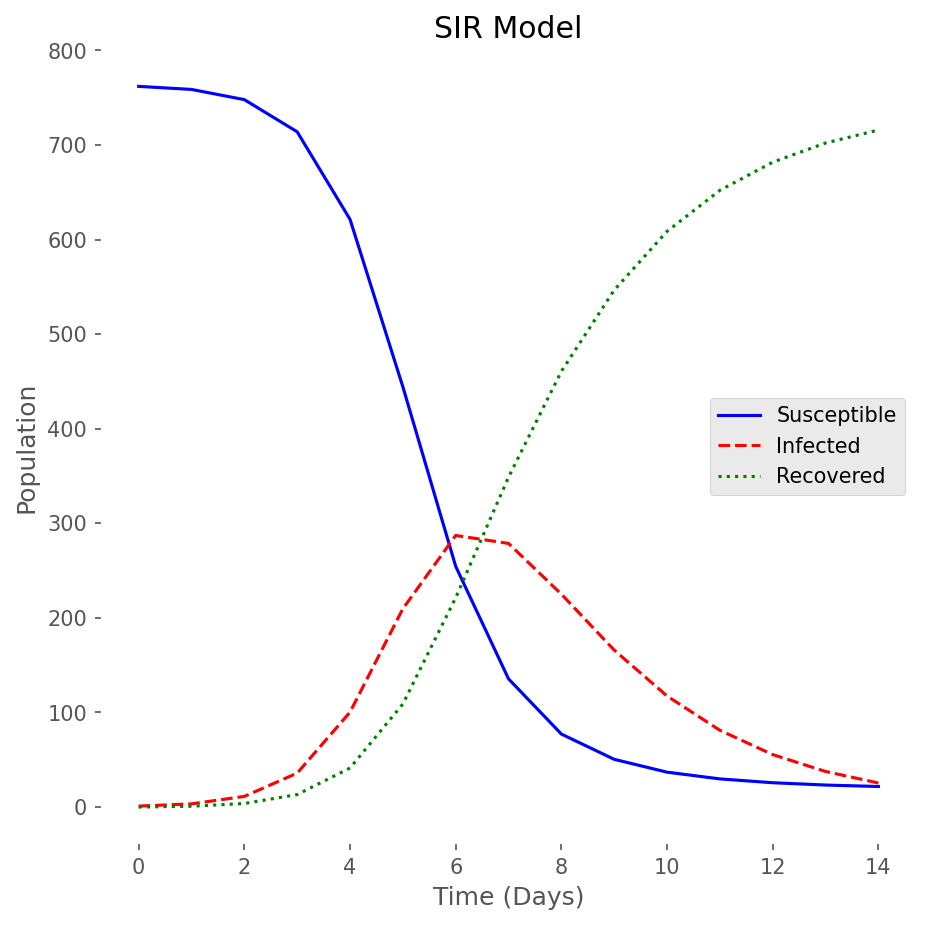
\includegraphics[scale=0.6]{SIR_graph.png}
\caption{Numeric Solution of SIR Model for Example Data}
\label{fig:SIR Model Numeric Solution}
\end{figure}

From the above graphs, it can be seen that, the susceptible population $S^{\prime}(t)$ is strictly decreasing with time, while the recovered population $R^{\prime}(t)$ is strictly increasing with time. But for the infectious population $I^{\prime}(t)$, the values increase at first and then decrease to zero finally. \\

Also, a phase portrait [34], [35], [36], [37] is a very convenient way to geometrically represent the trajectories of a dynamical system in a phase plane. \\

The phase portrait of the SIR model--- \\

\begin{figure}[H]
\centering
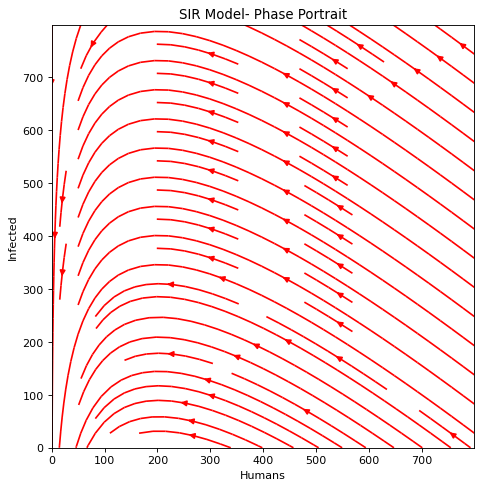
\includegraphics[scale=0.8]{SIR_PhasePortrait.png}
\caption{SIR Model- Phase Portrait}
\label{fig:SIR Model Phase Portrait}
\end{figure}

From the phase portrait, it can be seen that the SIR model is linearly stable and a disease free equilibrium exists. According to this very simple model, the survivability of human population in the long run is possible. \\

In Python code, solve\_ivp function from Scipy library [23] was used to solve the SIR differential equations and later plotted with matplotlib library [24]. Also, Numpy library [25] was used for some additional calculations. And for the phase portrait, streamplot [46] function was used. \\

Some more related examples regarding SIR model can be found at [26], [38], [39], [40], [41], [42], [43]. \\

Some studies on the recent Corona Virus Disease 2019 (COVID-19) using SIR model can be found at [44], [45]. \\

The source of the Python codes for this SIR model can be found in the Codes section of this thesis paper.










